\documentclass[]{standalone}
\usepackage[utf8]{inputenc}
\usepackage[english]{babel}
\usepackage{amsmath}
\usepackage{amsfonts}
\usepackage{amssymb}

\usepackage{graphicx}
%\usepackage[left=2cm,right=2cm,top=2cm,bottom=2cm]{geometry}

% Figures
\usepackage{tikz}
\usetikzlibrary{shapes,arrows}
\usetikzlibrary{positioning}
\usetikzlibrary{calc}
%\usepackage{chemfig}

% Tikz styles
\tikzstyle{reg} = [rounded rectangle, text width=2cm, fill=black!5, align=center, anchor=west,font=\sffamily\Large\bfseries, minimum height=1cm, inner sep=0]
\tikzstyle{rad} = [rounded rectangle, draw=none, text width=2cm, fill=red!10, align=center, anchor=west,font=\sffamily\Large\bfseries, minimum height=1cm, inner sep=0]
\tikzstyle{long} = [rounded rectangle, draw=none, text width=3.5cm, fill=black!5, align=center, anchor=west,font=\sffamily\Large\bfseries, minimum height=1cm, inner sep=0]   
\tikzstyle{add} = [scale=1.5, draw=none,fill=none,align=center]
\tikzstyle{emp} = [draw=none,fill=none]
\tikzstyle{ar} = [->,draw=black!70,line width=2]
\tikzstyle{ln} = [-,draw=black!70,line width=2]


\begin{document}
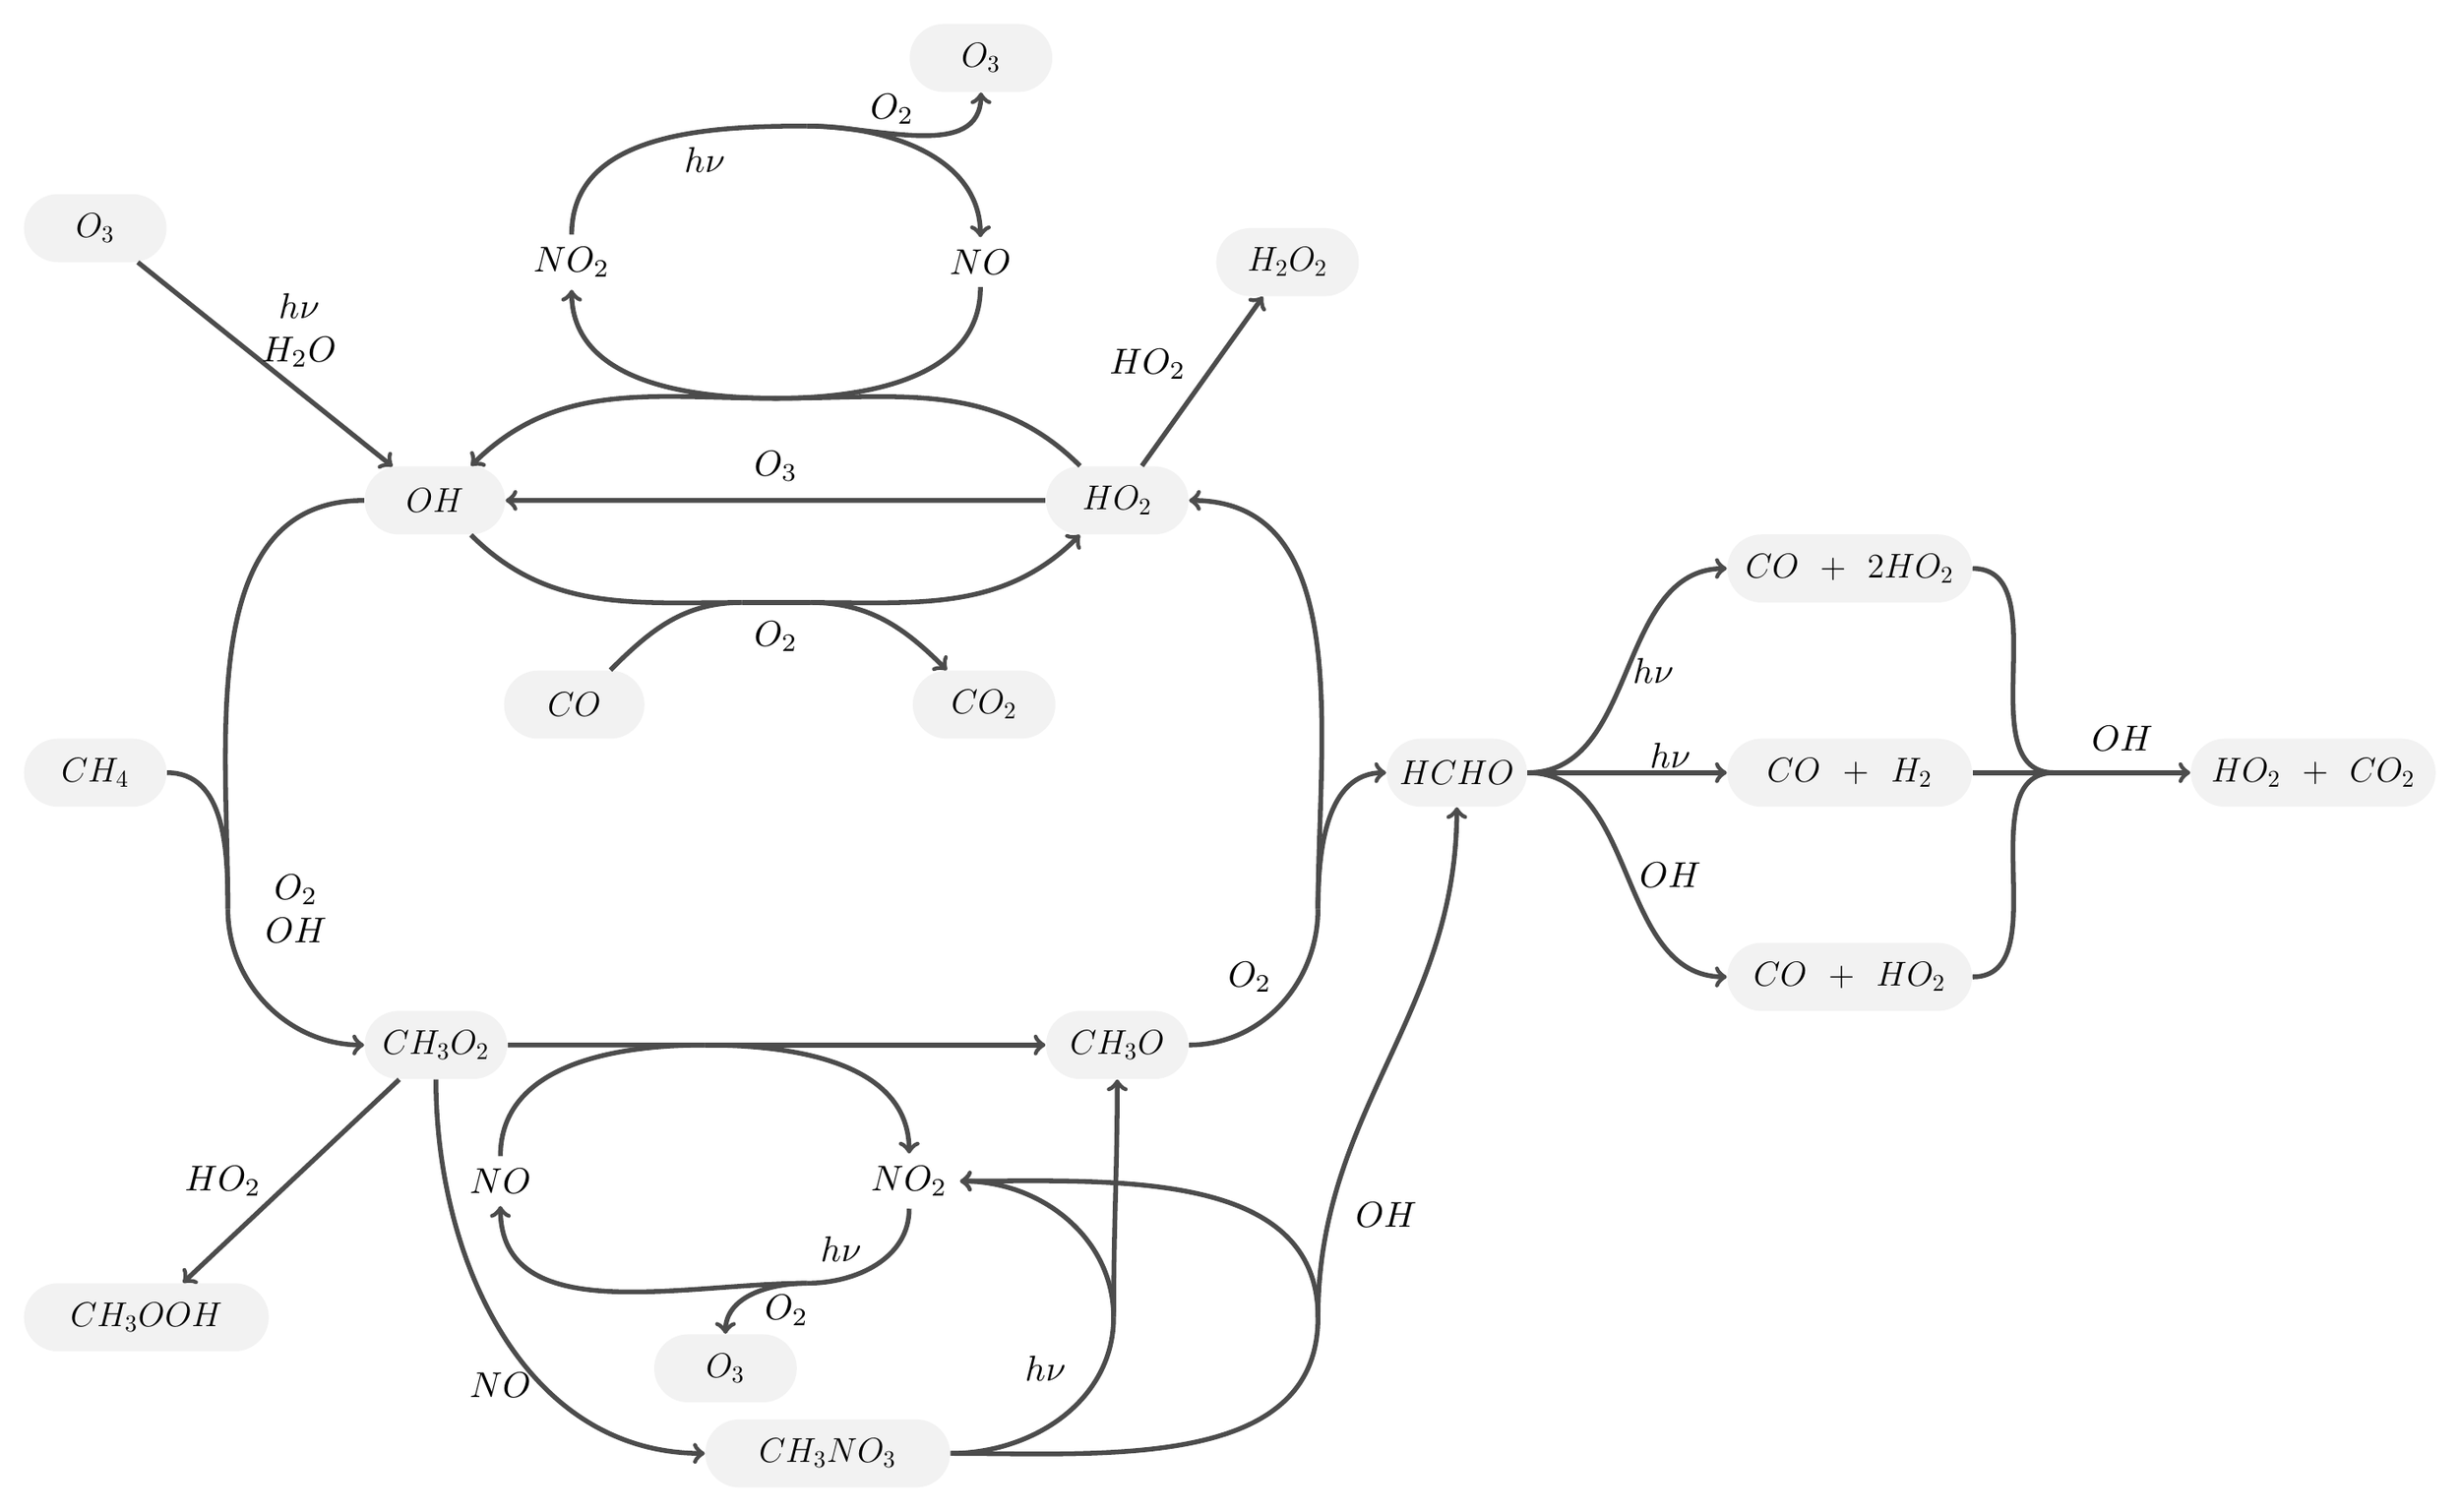
\begin{tikzpicture}[node distance = 4cm, auto]

% Nodes: big cycle: CH4-CH302-CH3NO3-CH3O-HCHO-HO2-OH-O3
\node[reg] (ch4) {$CH_4$};
\node[add](foo1_1) at (3,-2) {};
\node[add](foo1_2) at (4,-2) {$O_2$\\$OH$};
\node[reg] (ch3o2) at (5,-4){$CH_3 O_2$};
\node[reg] (oh) at (5,4){$OH$};
\node[long] (ch3ooh) at (0,-8){$CH_3OOH$};
\node[reg] (oz1) at (0,8){$O_3$};
\node[emp] (foo2) at ($(oz1)!.5!(oh)$){};
\node[reg] (ho2) at (15,4){$HO_2$};
\node[add] (oz_up) at ($(ho2)!.5!(oh) + (0,0.5)$){$O_3$};
\node[reg] (h2o2) at (17.5,7.5){$H_2O_2$};
\node[add] (ho2_) at (16.5,6){$HO_2$};
\node[emp] (nox_top) at ($(ho2)!.5!(oh) + (0,1.5)$){};
\node[reg] (ch3o) at (15,-4){$CH_3 O$};
\node[reg] (hcho) at (20,0){$HCHO$};
\node[emp] (foo5) at (19,-2){};
\node[long] (ch3no3) at (10,-10){$CH_3 NO_3$};
\node[add] (foo1_2) at (7,-9) {$NO$};
%\node[emp] (dep1) at (11,-12){};
%\node[add] (dep1_) at (10.3,-11.3){deposition};

%Nodes: Bottom NOx cycle + misc
\node[add] (no_1) at (7,-6){$NO$};
\node[add] (no2_1) at (13,-6){$NO_2$};
\node[emp] (nox_bottom) at ($(no_1)!.5!(no2_1)+(0,2)$){};
\node[emp] (foo7) at (11.5,-7.5){};
\node[add] (hv_11) at (12,-7){$h\nu$};
\node[reg] (o3_1) at (9.25,-8.75){$O_3$};
\node[add] (o2_1) at (11.2,-7.9){$O_2$};
\node[emp] (foo3) at (16,-8){};
\node[add] (hv_12) at (15,-8.75){$h\nu$};
\node[emp] (foo4) at (19,-8){};
\node[add] (oh_) at (20,-6.5){$OH$};
\node[add] (o2_) at (18,-3){$O_2$};

%Nodes: Top NOx cycle + misc
\node[add] (no2_2) at ($(ho2)!.5!(oh)+(-3,3.5)$){$NO_2$};
\node[add] (no_2) at ($(ho2)!.5!(oh)+(3,3.5)$){$NO$};
\node[add] (hv_2) at (10,9){$h\nu$};
\node[reg] (o3_2) at (13,10.5){$O_3$};
\node[add] (o2_2) at (12.75,9.75){$O_2$};
\node[emp] (foo6) at (11.5,9.5){};

%Nodes: CO & CO2
\node[reg] (co) at ($(ho2)!.5!(oh)+(-4,-3)$){$CO$};
\node[reg] (co2) at ($(ho2)!.5!(oh)+(2,-3)$){$CO_2$};
\node[emp] (cc_o2) at ($(ho2)!.5!(oh)+(0,-2.5)$){};
\node[emp] (cc_1) at ($(ho2)!.5!(oh)+(-0.5,-1.5)$){};
\node[emp] (cc_2) at ($(ho2)!.5!(oh)+(0.5,-1.5)$){};
\node[add] (cc_o2) at ($(ho2)!.5!(oh)+(0,-2)$){$O_2$};

%Nodes: HCHO decompostion
\node[long] (co_2ho2) at (25,3){$CO~+~2HO_2$};
\node[add] (hcho_hv1) at ($(hcho)!.5!(co_2ho2)$){$h\nu$};
\node[long] (co_h2) at (25,0){$CO~+~H_2$};
\node[add] (hcho_hv2) at ($(hcho)!.5!(co_h2)+(0.25,0.25)$){$h\nu$};
\node[long] (co_ho2) at (25,-3){$CO~+~HO_2$};
\node[add] (hcho_oh) at ($(hcho)!.5!(co_ho2)+(0.25,0)$){$OH$};
%\node[long] (hno3dep) at (25,-6){\small $CO~+~HO_2~+~HNO_3$\\ deposition?};
%\node[add] (hcho_no3) at ($(hcho)!.5!(hno3dep)$){$NO_3$};

%Nodes: after decomposition HO_2 + CO_2
\node[emp] (decomp) at ($(co_2ho2)!.5!(co_ho2)+(3,0)$){};
\node[long] (decomp2) at ($(decomp)+(2,0)$){$HO_2~+~CO_2$};
\node[add] (decomp_oh) at ($(decomp)+(1,0.5)$){$OH$};

% Connections: big cycle
\draw[ln] (oh.west) to [out=180,in=90](foo1_1.center);
\draw[ln] (ch4.east) to [out=0,in=90](foo1_1.center);
\draw[ar] (foo1_1.center) to [out=270,in=180](ch3o2.west);
\draw[ar] (ch3o2) to (ch3ooh);
\node[add](foo1) at ($(ch3o2)!.5!(ch3ooh) + (-1,0)$) {$HO_2$};
%\draw[ar] (oz1) to node[right]{$h\nu$}(foo2.north west);
\draw[ar] (oz1) to (oh);
\node[add] (o3_to_OH) at ($(oz1)!.5!(oh) + (0.5,0.5)$){$h\nu$\\ $H_2O$};
%\draw[ar] (foo2.south east) to node[right]{$H_2O$}(oh);
\draw[ar] (ho2) to (h2o2);
\draw[ln] (ho2.north west) to [out=135,in=0](nox_top.center);
\draw[ar] (nox_top.center) to [out=180,in=45](oh.north east);
\draw[ar] (ho2) to (oh);
\draw[ln] (ch3o2) to (nox_bottom.center);
\draw[ar] (nox_bottom.center) to (ch3o);
\draw[ar] (ch3o2.south) to [out=270,in=180](ch3no3.west);
\draw[ln] (ch3o.east) to [out=0,in=270](foo5.center);
\draw[ar] (foo5.center) to [out=90,in=0](ho2.east);
\draw[ar] (foo5.center) to [out=90,in=180](hcho.west);

% Connections: bottom NOx cycle + misc
\draw[ln] (no_1.north) to [out=90,in=180](nox_bottom.center);
\draw[ar] (nox_bottom.center) to [out=0,in=90](no2_1.north);
\draw[ln] (no2_1.south) to [out=270,in=0](foo7.center);
\draw[ar] (foo7.center) to [out=180,in=90](o3_1.north);
\draw[ar] (foo7.center) to [out=180,in=270](no_1.south);
\draw[ln] (ch3no3.east) to [out=0,in=270](foo3.center);
\draw[ar] (foo3.center) to [out=90,in=270](ch3o.south);
\draw[ar] (foo3.center) to [out=90,in=0](no2_1.east);
\draw[ln] (ch3no3.east) to [out=0,in=270](foo4.center);
\draw[ar] (foo4.center) to [out=90,in=270](hcho.south);
\draw[ar] (foo4.center) to [out=90,in=0](no2_1.east);
%\draw[ar] (ch3no3.south) -- (dep1.center);

% Connections: top NOx cycle
\draw[ln] (no_2.south) to [out=270,in=0](nox_top.center);
\draw[ar] (nox_top.center) to [out=180,in=270](no2_2.south);
\draw[ln] (no2_2.north) to [out=90,in=180](foo6.center);
\draw[ar] (foo6.center) to [out=0,in=90](no_2.north);
\draw[ar] (foo6.center) to [out=0,in=270](o3_2.south);

%Connections: CO & CO2
\draw[ln] (oh.south east) to [out=315,in=180](cc_1.center);
\draw[ln] (co.north east) to [out=45,in=180](cc_1.center);
\draw[ln] (cc_1.center) to [out=0,in=180](cc_2.center);
\draw[ar] (cc_2.center) to [out=0,in=225](ho2.south west);
\draw[ar] (cc_2.center) to [out=0,in=135](co2.north west);

%Connections: HCHO decomp
\draw[ar] (hcho.east) to [out=0,in=180](co_2ho2.west);
\draw[ar] (hcho.east) to [out=0,in=180](co_h2.west);
\draw[ar] (hcho.east) to [out=0,in=180](co_ho2.west);
%\draw[ar] (hcho.east) to [out=0,in=180](hno3dep.west);

\draw[ln] (co_2ho2.east) to [out=0,in=180](decomp.center);
\draw[ln] (co_h2.east) to [out=0,in=180](decomp.center);
\draw[ln] (co_ho2.east) to [out=0,in=180](decomp.center);
\draw[ar] (decomp.center) to [out=0,in=180](decomp2.west);


\end{tikzpicture}

\end{document}